\documentclass{article}
\usepackage[utf8]{inputenc}
\usepackage{todonotes}
\usepackage{float}
\usepackage{graphicx}
\usepackage{biblatex}
\usepackage{hyperref}

\usepackage{listings}

\lstset{%
  language = Octave,
  backgroundcolor=\color{white},   
  basicstyle=\footnotesize\ttfamily,       
  breakatwhitespace=false,         
  breaklines=true,                 
  captionpos=b,                   
  commentstyle=\color{gray},    
  deletekeywords={...},           
  escapeinside={\%*}{*)},          
  extendedchars=true,              
  frame=single,                    
  keepspaces=true,                 
  keywordstyle=\color{orange},       
  morekeywords={*,...},            
  numbers=left,                    
  numbersep=5pt,                   
  numberstyle=\footnotesize\color{gray}, 
  rulecolor=\color{black},         
  rulesepcolor=\color{blue},
  showspaces=false,                
  showstringspaces=false,          
  showtabs=false,                  
  stepnumber=2,                    
  stringstyle=\color{orange},    
  tabsize=2,                       
  title=\lstname,
  emphstyle=\bfseries\color{blue}%  style for emph={} 
} 

%% language specific settings:
\newcommand\YAMLcolonstyle{\color{red}\mdseries}
\newcommand\YAMLkeystyle{\color{black}\bfseries}
\newcommand\YAMLvaluestyle{\color{blue}\mdseries}
\lstdefinestyle{yml}{%
    keywords={true,false,null,y,n},
    keywordstyle=\color{darkgray}\bfseries,
    basicstyle=\YAMLkeystyle,                                 % assuming a key comes first
    sensitive=false,
    comment=[l]{\#},
    morecomment=[s]{/*}{*/},
    commentstyle=\color{purple}\ttfamily,
    stringstyle=\YAMLvaluestyle\ttfamily,
    moredelim=[l][\color{orange}]{\&},
    moredelim=[l][\color{magenta}]{*},
    moredelim=**[il][\YAMLcolonstyle{:}\YAMLvaluestyle]{:},   % switch to value style at :
    morestring=[b]',
    morestring=[b]",
    literate =    {---}{{\ProcessThreeDashes}}3
                {>}{{\textcolor{red}\textgreater}}1     
                {|}{{\textcolor{red}\textbar}}1 
                {\ -\ }{{\mdseries\ -\ }}3,
    title={ docker-compose.yml}
}

\addbibresource{report/bibliography.bib}

\title{
\textsc{\huge IT-University of Copenhagen}\\[1cm]\\
\textsc{\LARGE \textbf{DevOps Minitwit - Group A}}\\[1cm]\\
}

\author{
Martin Meldgaard Holst - (mmho@itu.dk),\\
Hampus Michael W. Iversen - (haiv@itu.dk), \\
Niels-Frederik Brinck - (nieb@itu.dk),\\
Emil Knudsen - (emkn@itu.dk),\\
Marcus Norton Quistgaard - (marq@itu.dk)}
\begin{document}
\maketitle
\begin{center}
\textsc{Course code: KSDSESM1KU}
\end{center}

\newpage
\tableofcontents
\newpage

\section{System's Perspective}
\newpage
\section{Process' perspective}

\subsection{Team Organization and Interaction}
The team created a Discord channel to function as the main communication channel throughout the project. Here, the team met each Monday after the lecture to discuss what work had been completed since last week, what work had to be completed by the end of the current week, and who should do which tasks. \\
The team used Jira's Kanban Board feature\cite{jira} to gain a better overview of the various tasks. The Kanban consisted of the following columns: "To Do", "In Progress", and "Done". Hence, the team could move the tasks to the corresponding status of its progress, such that the state was visible to the rest of the team members.

\subsection{CI/CD Pipeline and Tools} \label{CI/CD}
The CI/CD pipeline uses GitHub actions, Travis CI, ESLint, SonarCloud, and Semantic Release. GitHub actions are run on both the Develop and main branch when a pull request or push to the repository is made. \\

ESLint is used through the GitHub action \textit{stefanoeb/eslint-action@1.0.2} \cite{eslint-action} and is performing static code analysis by checking line indentation, unused variables, props passed to React components, etc. Travis CI is integrated into the MiniTwit repository and is used to run all unit tests within the MiniTwit/API folder \cite{travis-ci}. SonarCloud is also used to perform static code analysis and checks code smells such as code duplication exceeding 4\%. It also scans for potential security vulnerabilities \cite{sonarcloud}.

\subsubsection{Pull Request}
On a pull request, the Travis CI, SonarCloud, and ESLint GitHub action are all being run. If they all pass the developers are allowed to perform the merge.

\subsubsection{Push}
On a push to the main or Develop branch, the \textit{Build and Push} GitHub action is run. The jobs build the Frontend, API, and Sim-API Docker images and push them to Dockerhub. Once all three jobs have finished, a fourth job is started, which SSHs into the swarm manager droplet on Digital Ocean. This job updates the corresponding running services in the swarm by using the \textit{docker service update --image name-of-image} command. The SSH action is \textit{appleboy/ssh-action@master}\cite{ssh-action}. Below is an image from the GitHub action log showing the four jobs:

\begin{figure}[H]
    \centering
    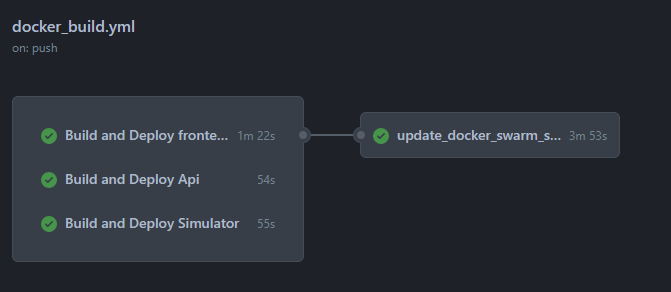
\includegraphics[width=1\linewidth]{report/images/build-and-deploy-action.png}
    \caption{Build and deploy action dependency graph}
    \label{fig:build-and-deploy}
\end{figure}

Furthermore, a GitHub action with the name \textit{Create Release} running \textit{Semantic Release} will act on any push to the main branch with a commit name with the prefix \textit{fix}, \textit{feat} or \textit{BREAKING CHANGE}. If the commit's name fulfills the prefix, the \textit{Semantic Release} will create a new release on the main branch \cite{semantic-release}.\\
\\
A last action named \textit{Latex to PDF} is run in the \textit{latex\_to\_pdf.yml} file, which compiles the \textit{main.tex} file in the Minitwit/report/directory folder. This action compiles the \textit{main.tex} file using the GitHub action \textit{xu-cheng/latex-action@v2} \cite{latex-action} and outputs it as \textit{report.pdf}. It then commits and pushes the new file to the main branch in the same directory.

\subsection{Organization of Repository}
The MiniTwit application was built using a mono-repository on GitHub. The structure in the repository consisted of a sub-folder for the API (API for the front end and the Simulator API), a sub-folder for the Frontend React Application, and a sub-folder for the report written in Latex. 

\subsection{Applied Branching Strategy}
The team applied the task-branching strategy\cite{branching} together with having both a Main and Develop branch. The Develop branch was initially a mirror of the Main branch and is where new functionality is developed and tested. Once a task is created on Jira and a team member has been assigned to develop it, the developer will create a branch with the task name off of the Develop branch. Once completed and tested successfully, the branch is merged into Develop. Finally, Develop was merged into Main once a week. However, this was not happening weekly in the first weeks of the project due to the team being behind schedule. 

\subsection{Applied Development Process and Tools Supporting It}
The team tried to use pair-programming in an informal manner as much as possible, as opposed to assigning each member with their own task. Pair programming was preferred to allow most possible members to get hands-on experience with the various DevOps themes and to enhance code quality. To facilitate pair-programming, the team utilized Discord's screen sharing functionality as well as Visual Studio Code's Live Share functionality\cite{live_share}. While screen sharing functionality is self-explanatory, the Live Share functionality provided a way for multiple developers to navigate the documents simultaneously. 

\subsection{Monitoring and Logging}

\subsubsection{Metrics Collection}
%How do we monitor
The Prometheus container uses the \textit{local} network which is configured to use an overlay driver in the \textit{docker-compose.yml}:

\begin{figure}[H]
    \centering
    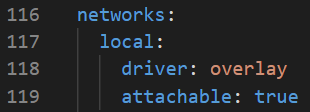
\includegraphics[width=0.4\linewidth]{report/images/LocalNetwork1.png}
    \caption{code snippet from Minitwit/docker-compose.yml}
    \label{fig:docker-compose-overlay}
\end{figure}
\noindent See appendix \ref{appendix:docker-compose} for the full compose file.\\
The services to be scraped are also running on the \textit{local} network.\\
This network configuration allows Prometheus to retrieve the virtual IP addresses of all of the api and sim-api service replicas running in the Docker swarm. Prometheus's scraping job is configured in the \textit{Minitwit/prometheus.yml}:

\begin{figure}[H]
    \centering
    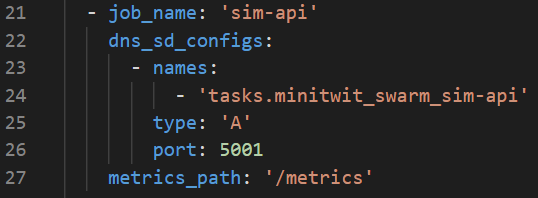
\includegraphics[width=0.66\linewidth]{report/images/LocalNetwork2.png}
    \caption{code snippet from Minitwit/prometheus.yml}
    \label{fig:prometheus-scraping}
\end{figure}
\noindent See appendix \ref{appendix:prometheus-config} for the full configuration file.\\
Here, the sim-api job scrapes all sim-api tasks/replicas by executing a DNS query to retrieve their IP and pull the metrics with the specified \textit{metrics\_path} endpoint.\\
As of the current setup, only the sim-api service is being scraped and not the api service.
The monitoring setup uses a pull based monitoring setup where Prometheus pulls the metrics from the services and Grafana pulls the metrics from Prometheus.\\

Figure \ref{fig:back-end-depencency-diagram} shows that both the API and sim-API use the prom-client library to passively monitor endpoint requests and responses by "sniffing".
Prom-client is used for the whitebox monitoring as part of the API's middleware to monitor the total requests and responses and the individual endpoints and response codes.
\\

%What precisely do we monitor
As seen in the figure \ref{fig:Monitoring1}, the Grafana dashboard displays graphs for the total amount of requests and responses as well as more precise counters for the requests and responses of each endpoint in the last hour. Furthermore, figure \ref{fig:Monitoring2} shows the average response time of some of the endpoints monitored to keep track of bottlenecks.

\begin{figure}[H]
    \centering
    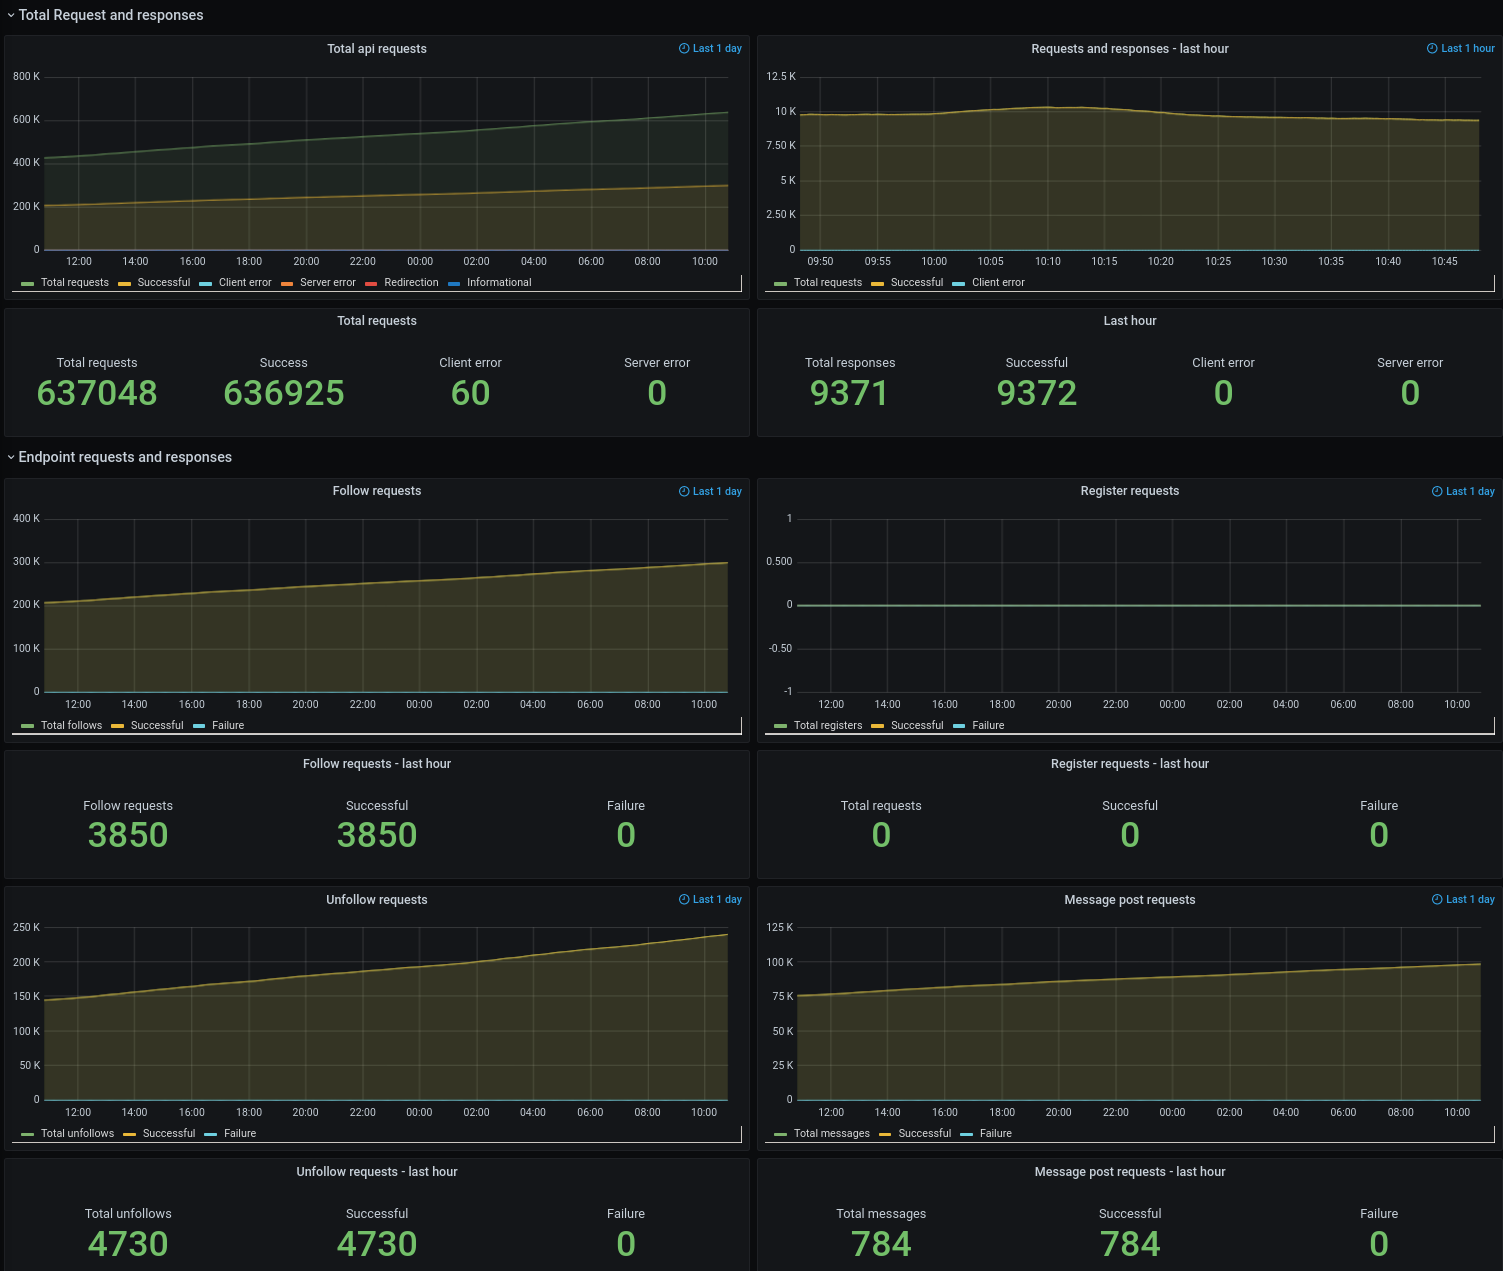
\includegraphics[width=1\textwidth]{report/images/MonitoringRequest.png}
    \caption{Request/response monitoring. \href{https://github.com/Niels-Frederik/MiniTwit/blob/main/report/images/MonitoringRequest.png}{Click here for full size image}}
    \label{fig:Monitoring1}
\end{figure}

\begin{figure}[H]
    \centering
    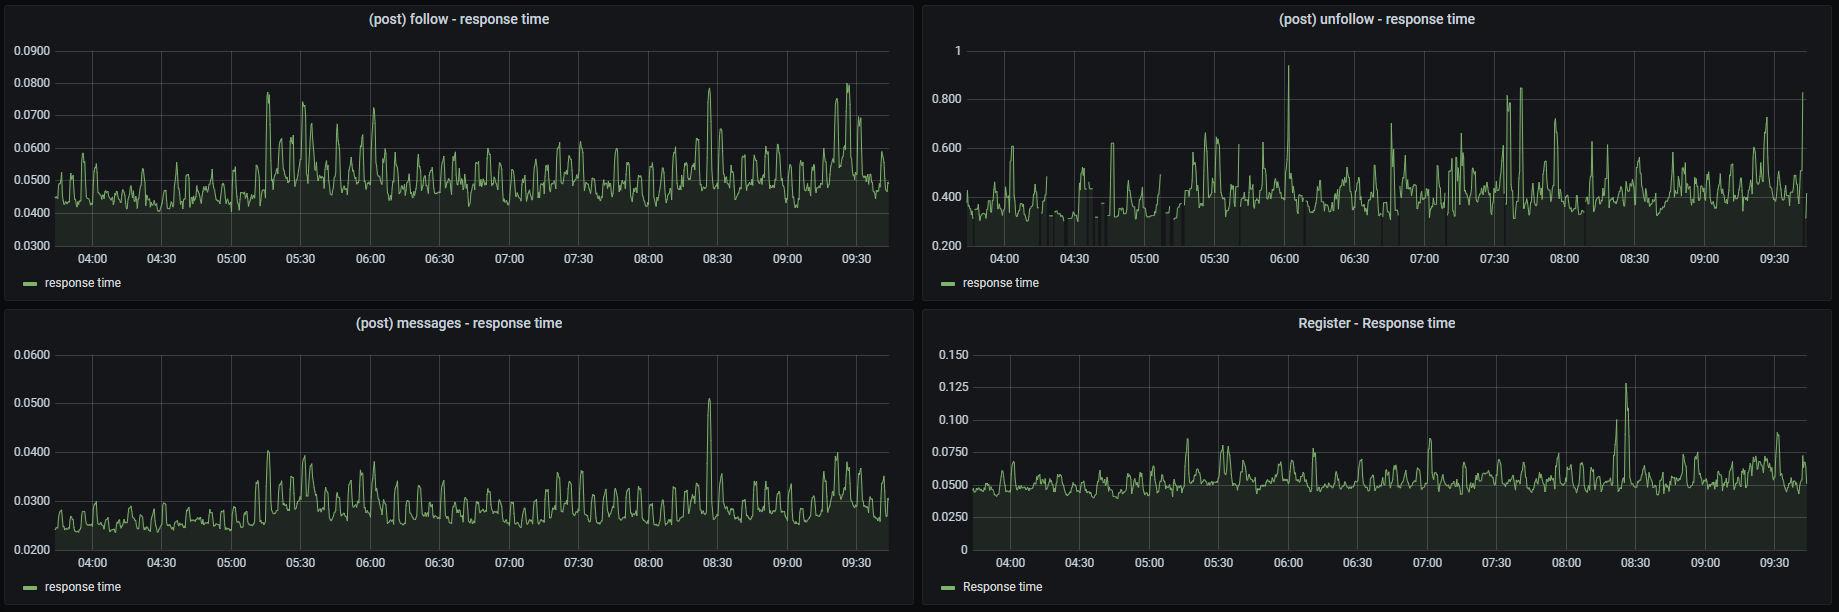
\includegraphics[width=1\textwidth]{report/images/grafana-response-times.png}
    \caption{Average response time monitoring. \href{https://github.com/Niels-Frederik/MiniTwit/blob/main/report/images/grafana-response-times.png}{Click here for full size image}}
    \label{fig:Monitoring2}
\end{figure}


The dashboard allows for a quick overview of user activity as well as average response times.
This makes it easy to monitor the number of errors compared to requests, the type of errors, the endpoints which fail, and potential bottlenecks.
%More or less load as well as which day registers happened (in test simulation)
%quick and easy overview of which endpoints fails and how much
%Endpoints responses... Like do users or the server cause errors in specific endpoints
%Allowed us to easily see how missing users from downtime cause user errors in endpoints...
%Maybe even downtime


%Snak om at vi intet infrastructure har, men hvordan vi kunne have gjort det 


\subsubsection{Log Collection and Aggregation}
The system uses a Loki/Promtail/Grafana stack for logging. A Loki driver is installed on both the nodes in the docker swarm service with the following command:

\begin{verbatim}
    docker plugin install grafana/loki-docker-driver:latest
    --alias loki --grant-all-permissions
\end{verbatim}

Furthermore, the \textit{/etc/docker/daemon.json} file on both nodes is modified, which allows for all docker containers to redirect their logs to the Loki endpoint via the Loki driver.

\begin{verbatim}
    {
    "debug" : true,
    "log-driver": "loki",
    "log-opts": {
        "loki-url": "http://161.35.214.217/loki/api/v1/push"
    }
}
\end{verbatim}

This allows for aggregating logs from all nodes in the docker swarm stack, which the Grafana dashboard can query and visualize. Lastly, a Promtail container is deployed to access locally stored logs. Promtail is not currently utilized on the Grafana logging dashboard but can be useful for accessing specific logs.\\

\noindent
This stack is chosen for many different reasons:
\begin{itemize}
    \item Requires significantly less memory compared to ELK/EFK stack
    \item Utilizing Grafana for visualization, which is already used by Prometheus
    \item Easy setup and integration with docker swarm
\end{itemize}

Furthermore, the collection of logs have utilized the Winston and Express-Winston library in order to provide an easier way to maintain how logs are stored and formatted.\cite{winston} As an example, the following CustomLogFormat has been created:
\begin{verbatim}
    const customLogFormat = printf(({message, level, timestamp}) => {
        return `${timestamp} ${level}: ${message}`
    });
    
    const customLogger = createLogger({
        format: combine(timestamp(), customLogFormat),
        transports: [new transports.Console()],
    });
\end{verbatim}
This provides a log format to be used which shows the time-stamp of the log, the logging level, and the log message. Hence, the logs get a common syntax, and if a change is needed in the syntax it happens in a single place.
\\\\
This also allows for splitting the logs into 3 different levels; information, warnings, and errors. It was chosen to log requests to each endpoint, either resulting in a successful log, a warning, or an error.
\noindent
For the dashboard it was chosen to visualize the information logs, error logs, and warning logs independently, to provide an easy overview of processes happening in the system. This dashboard can be seen in figure \ref{fig:loggingDashboard} below.\\

\begin{figure}[H]
    \centering
    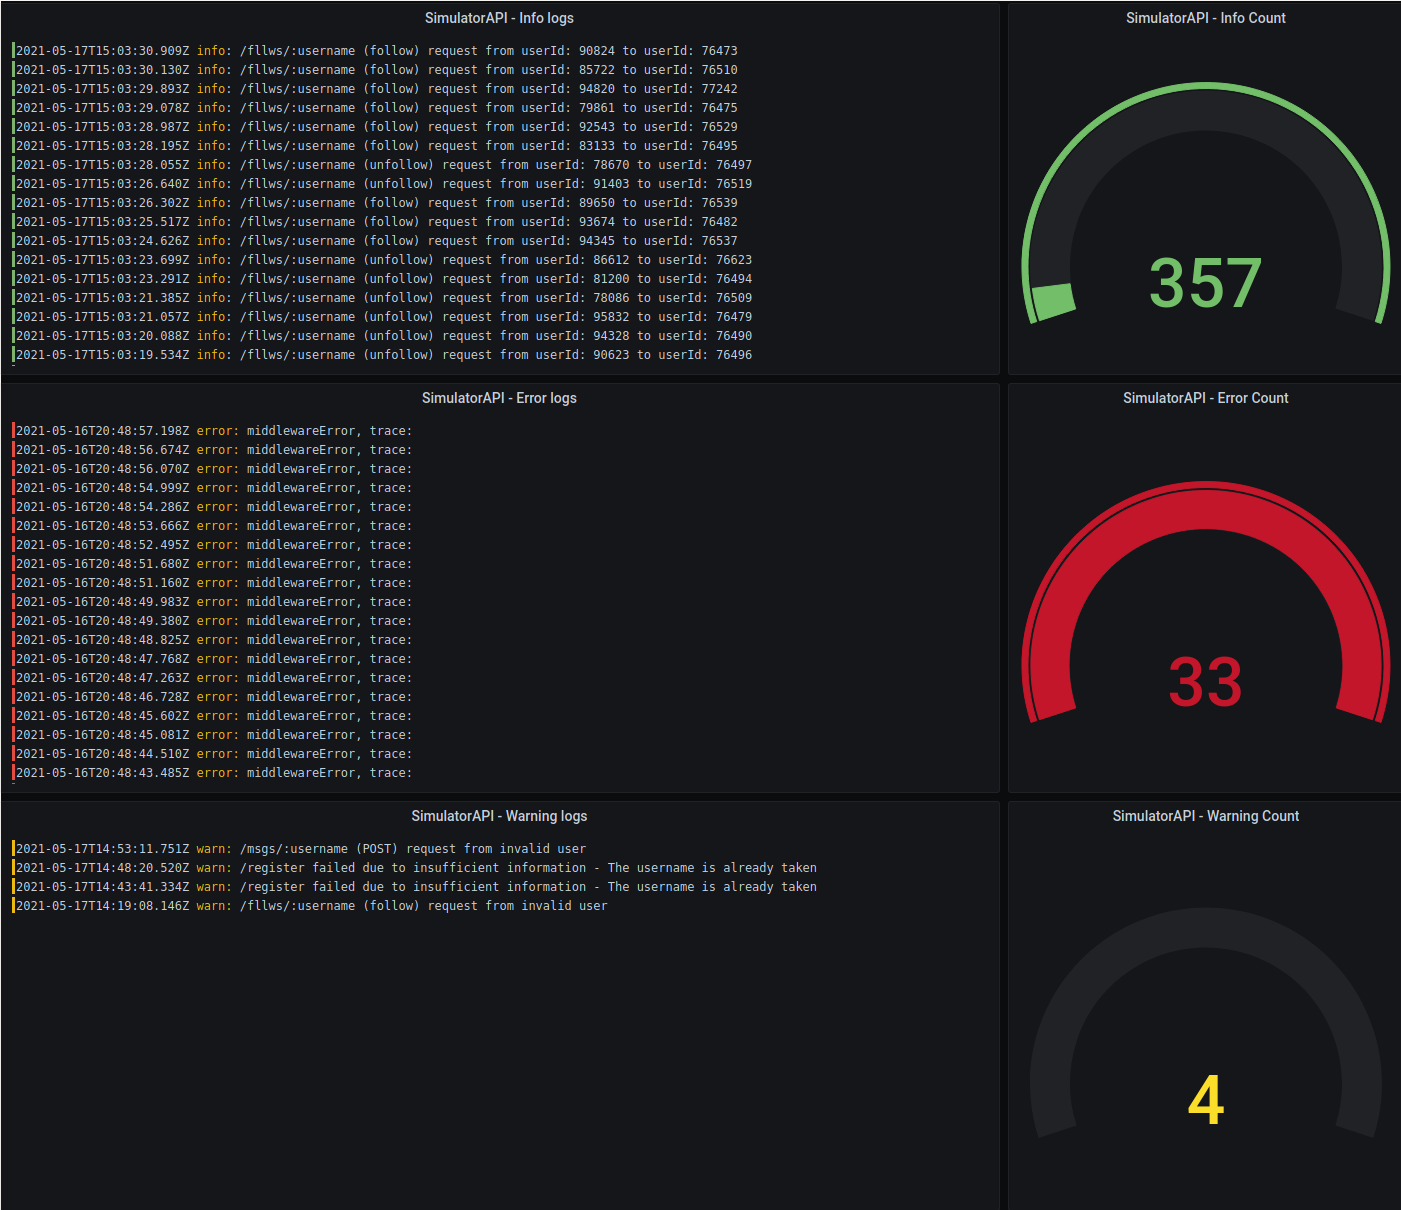
\includegraphics[width=\textwidth]{report/images/2021-05-17-170456_1401x1210_scrot.png}
    \caption{Logging dashboard from Grafana. \href{https://github.com/Niels-Frederik/MiniTwit/blob/main/report/images/2021-05-17-170456_1401x1210_scrot.png}{Click here for full size image}}
    \label{fig:loggingDashboard}
\end{figure}


\subsubsection{Alerts}\label{section:alerts}
To allow for a quick response to possible errors, an alerting rule has been implemented in Grafana. This is integrated with the team's Discord channel, meaning when an error is identified, a message is sent to the discord server. Figure \ref{fig:grafana-alert} below shows an example of an alert sent by Grafana to the team's discord server:

\begin{figure}[H]
    \centering
    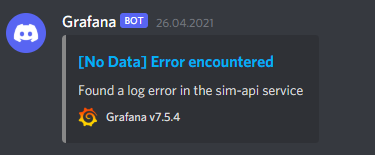
\includegraphics[width=0.6\linewidth]{report/images/grafana-alert.png}
    \caption{Grafana alert in discord}
    \label{fig:grafana-alert}
\end{figure}

\subsection{Brief Results of the Security Assessment}
Analyzing our system in regards to the OWASP top 10 web application security risks, we find that we break point 10: Insufficient logging and monitoring. This is also discussed in section \ref{section:llmonitoring}. Furthermore, the security of the system could be improved by implementing backups. At the current state, if the database is hacked all data would be gone. Lastly, some secrets have not been properly protected. In the GitHub history, some old secrets can be found and possibly exploited. These secrets were also at times communicated through unsafe communication channels such as Discord.\\   

A basic pentesting of the system has been performed. NMAP was used to investigate open ports but showed no exploitable weaknesses. Port 22 was running OpenSSH 8.2p1, which could allow for a brute force password attack. However, multiple steps were taken to prevent this, meaning it was no threat. These included limiting SSH access to the use of RSA keys and using a timeout after 6 failed attempts. Both DIRB and DIRBUSTER were run to check for directories or files, but none were found. Lastly, the site was checked for cross-site scripting and SQL injection attacks, but no vulnerabilities were found.


\subsection{Applied Strategy for Scaling and Load Balancing}
As already mentioned, the system is hosted in Docker swarm mode with two nodes running on their own droplets in the network. The docker swarm scales horizontally, as more worker nodes running on their own physical machine can join the swarm if the swarm was to be scaled. \\
\\
The default swarm setup implements load balancing out of the box. The load balancer decides which of the running instances, of the requested service, the request should end up at\cite{docker-ingress}. This is seen in figure \ref{fig:arcitechture-overview} where an incoming request to the load balancer on the \textit{minitwit-webserver} droplet can be redirected to a container running within the \textit{Minitwit} component of the \textit{production-worker} droplet.

\subsubsection{Updating the Swarm}
The swarm is configured to use rolling updates with \textit{--update-order} set to \textit{start-first}. For each service, an updated version is instantiated and monitored for 5 seconds before it is decided to be running successfully. Once running, the old instance of the service is shut down. This rolling update strategy is run for each service for each replica. See appendix \ref{appendix:docker-compose} for the full docker-compose.yml.\\
The start-first approach was chosen to guarantee that at least the desired amount of replicas are always run during updates.
\newpage
\section{Lessons Learned Perspective}
\newpage
\section{Appendix}

\subsection{docker-compose.yml}\label{appendix:docker-compose}
\lstinputlisting[style=yml, title=docker-compose.yml]{docker-compose.yml}

\newpage

\subsection{Prometheus.yml}\label{appendix:prometheus-config}
\lstinputlisting[style=yml, title=prometheus.yml]{prometheus.yml}

\newpage
\printbibliography
\end{document}
